\documentclass[a4paper,10pt]{scrartcl}
\usepackage[utf8]{inputenc}
\usepackage[T1]{fontenc}
\usepackage[naustrian]{babel}
\usepackage{lmodern}
\usepackage{graphicx}
\usepackage{hyperref}

%\usepackage{tabularx}
%\usepackage{amsmath}

%opening
\title{HCI Meilenstein 3}
\subtitle{Elektronisches Curriculum}
\author{Team 1 \\Pascal Attwenger, Philipp Hiermann, Sandra Markhart}

\begin{document}

\maketitle

\section{Usability Test Aufgaben}

\subsection{Aufgabe 1}

\noindent\makebox[\textwidth]{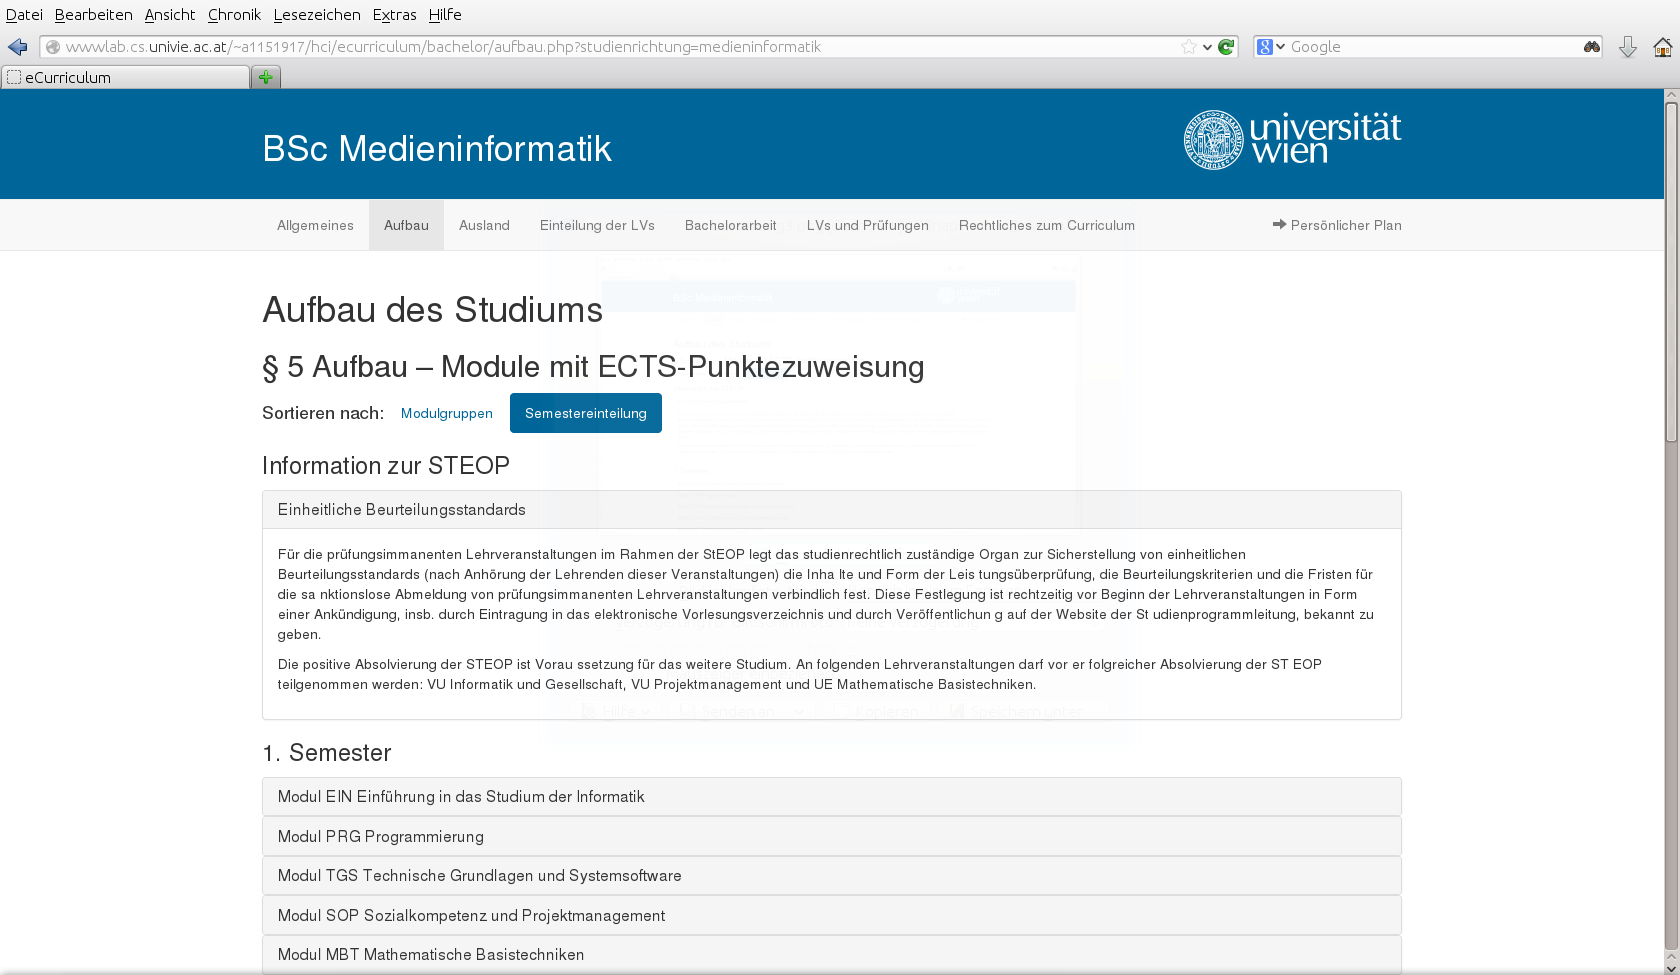
\includegraphics[width=\textwidth]{./aufgabe1.png}}
\medskip

\subsubsection*{Ziel:}
 
Der User soll herausfinden welche Fächer er im 1. Semester absolvieren muss und kann.
 
\subsubsection*{Beschreibung:}

Du fängst nächstes Semester an Medieninformatik zu studieren. Für welche Fächer sollst du dich anmelden?
 
\subsection{Aufgabe 2}

\noindent\makebox[\textwidth]{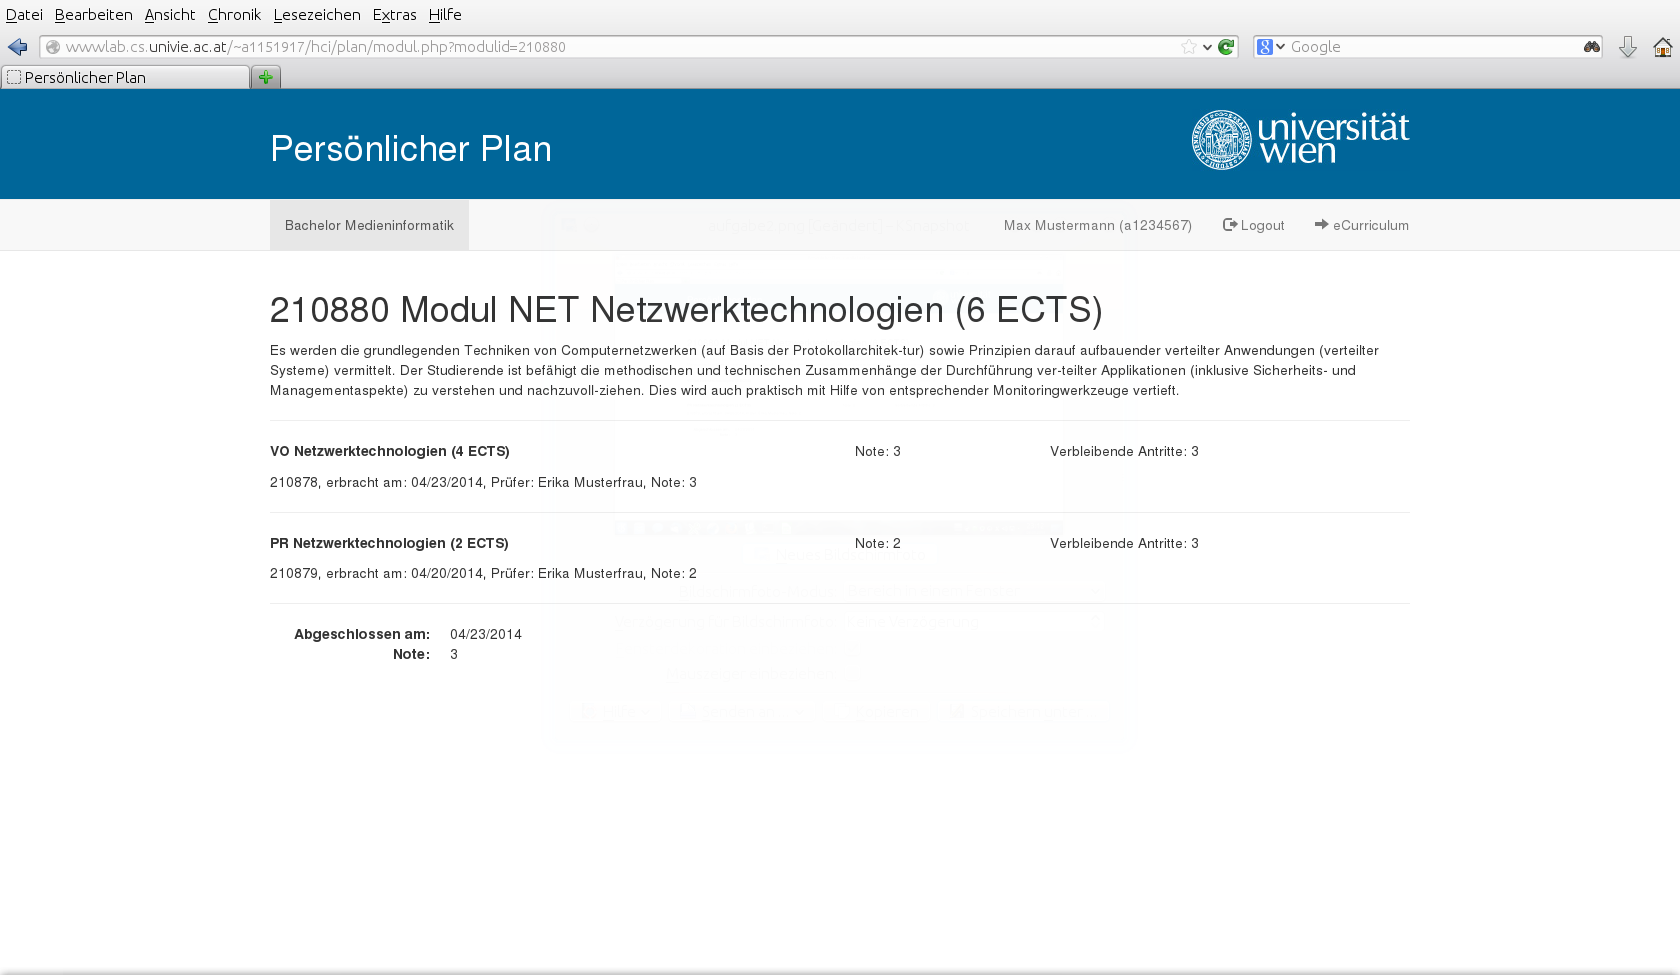
\includegraphics[width=\textwidth]{./aufgabe2.png}}
\medskip


\subsubsection*{Ziel:}

Der User soll seine Note abfragen.

\subsubsection*{Beschreibung:}

Du hast vor 2 Wochen die Vorlesungsprüfung zu VO Netzwerktechnologien abgelegt. Hast du bereits eine Note erhalten? Wenn ja welche?

\subsection{Aufgabe 3}

\noindent\makebox[\textwidth]{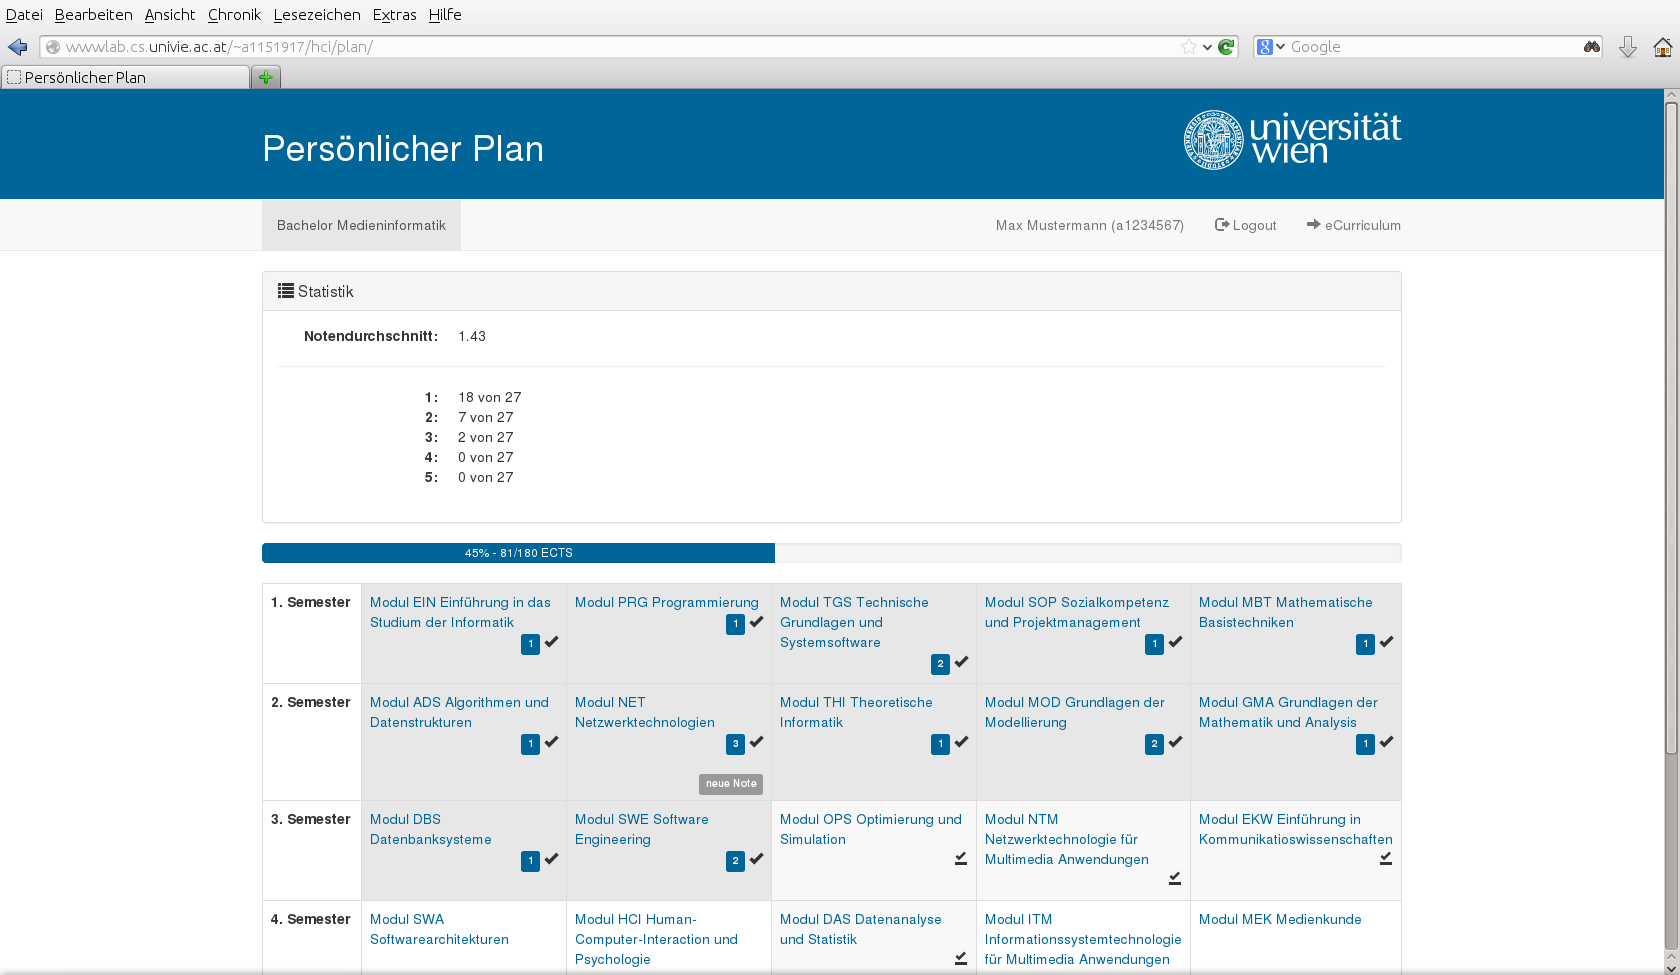
\includegraphics[width=\textwidth]{./aufgabe3.png}}
\medskip

\subsubsection*{Ziel:}

Der User soll seinen Notendurchschnitt herausfinden.

\subsubsection*{Beschreibung:}

Du studierst an der Universität Wien und willst wissen ob du dich für ein Leistungsstipendium eignest. Das Stipendium verlangt einen Notendurchschnitt von
1,8. Kannst du ein Leistungsstipendium erhalten?

\section{Interviewleitfaden}

\subsection{Vorinterview}

Zu Beginn des Interviews werden Fragen in schriftlicher Form zu den Erfahrungen und den Erwartungen an ein solches System gestellt.

\begin{itemize}
 \item Was sind deine Erfahrungen mit den aktuellen IT-Systemen im Studium? (univis, TISS, etc.)
 \item Was sind deiner Meinung nach die größten Schwächen dieser Systeme?
 \item Was würdest du dir von einem neuem System erwarten?
\end{itemize}

\subsection{Fragen nach der Aufgabe}

Als nächstes folgt die Durchführung der definierten Usability-Aufgaben. Fragen werden je nach Aufgabe mündlich gestellt, und die Antworten dazu notiert.

\subsubsection*{Ad Aufgabe 1}

\begin{itemize}
 \item Ist dir klar, was die StEOP generell ist?
 \item Angenommen, du würdest nur die unbedingt vorausgesetzten StEOP-Fächer belegen wollen -- welche wären das?
 \item Angenommen, du würdest alles belegen wollen, was im ersten Semester überhaupt möglich ist -- welche Fächer wären jetzt zusätzlich dabei?
 \item Was hältst du von der Darstellungsart, bei der immer nur genau ein Modul angezeigt wird?
 \item Vergleiche die Sortierung nach Modulgruppen mit der nach Semestereinteilung -- welche erscheint dir vernünftiger, und wieso?
 \item Wirf noch einen Blick auf die anderen Rubriken des eCurriculums (Allgemeines, Ausland, etc.) -- macht diese Aufteilung so für dich Sinn? Was würdest du evtl. anders gruppieren?
 \item Hast du noch andere Anmerkungen zu dieser Oberfläche?
\end{itemize}

\subsubsection*{Ad Aufgabe 2}

\begin{itemize}
 \item Ist dir klar, was es mit dem ``Persönlichen Plan'' auf sich hat?
 \item Ist dir der Unterschied zwischen Modulnote und LV-Note bewusst?
 \item Was bedeuten die kleinen Symbole (``Hakerl'') in der Tabellen-Übersicht?
 \item Kann diese Art der Darstellung die Listen-Ansicht der Prüfungsleistungen ersetzen oder nur ergänzen?
 \item Kannst du dir vorstellen, dass diese Art des Semesterplans auch für dein Studium möglich wäre? Wo wären eventuelle Probleme?
 \item Hast du noch andere Anmerkungen zu dieser Oberfläche?
\end{itemize}

\subsubsection*{Ad Aufgabe 3}

\begin{itemize}
 \item Findest du die automatische Berechnung des Notenschnitts sinnvoll? Wozu braucht man diese Information?
 \item Welche anderen Statistiken fändest du praktisch?
 \item Was hältst du von der Studienfortschrittsanzeige?
 \item Hast du noch andere Anmerkungen zu dieser Oberfläche?
\end{itemize}

\subsection{Abschlussinterview}

Zum Abschluss wird ein Fragebogen in schriftlicher Form vorgelegt, der von der interviewten Person auszufüllen ist. 
Für den Fragenbogen wurde ein Teil der Fragen aus dem Fragebogen 
der ISONORM 9241/110-S adaptiert.

\begin{itemize}

 \item Was sind deine allgemeinen Eindrücke vom System?
 \begin{itemize}
    \item Das System erfordert wenig Zeit zum Lernen.
 \end{itemize}
 \item Wie gut konntest du mit diesem System die Aufgaben bewältigen?
 \begin{itemize}
    \item Das System bietet alle Funktionen um die anfallenden Aufgaben zu bewältigen.
    \item Das System ist gut auf die im Studium zu bewältigenden Aufgaben zugeschnitten.
 \end{itemize}
 \item Wie gut konntest du dich orientieren?
 \begin{itemize}
    \item Das System liefert Informationen darüber, welche Eingaben zulässig oder nötig sind.
    \item Das System erleichtert die Orientierung durch eine einheitliche Gestaltung.
    \item Das System lässt sich nach einem einheitlichen Prinzip bedienen.
 \end{itemize}
 \item Was hat dir besonders gut/schlecht gefallen?
 \item Wurden deine Erwartungen an das System erfüllt?
 \item Hast du Verbesserungsvorschläge?
\end{itemize}

\subsection{Fragebogen}

Für das Vorinterview und das Nachinterview liegen die Fragen als Fragebogen vor, welcher schriftlich ausgefüllt werden kann.

\begin{description}
 \item[Datei auf cewebs:]Meilenstein 3 - Team 1 - Fragebogen
\end{description}

\section{Interviews}

\subsection*{Interview 1}

Der Interviewte ist 27, männlich und studiert im 6. Semester Medieninformatik.

\subsubsection*{Vorinterview}

Da der Interviewte auch an der Uni Wien studiert verwendet er das univis. Er ist der Meinung, dass das System sehr schlecht zu bedienen ist und mit den Konzepten
aus den 90er jahren entwickelt wurde. Von einem neuem System erwartet er sich eine bessere Bedienbarkeit des Systems und die Unterstützung bei der Anmeldung
anstatt, dass diese erschwert wird.

\subsubsection*{Aufgabe 1}

Der Interviewte 1 würde sich für alle 5 Module anmelden.

\begin{itemize}

\item Ist dir klar, was die StEOP generell ist? \\

Der Interviewte ist der Meinung, dass das klar ist, da es da steht. Evtl. sollte jedoch die Information zur Steop gleich zu Beginn aufgeklappt sein, da diese Information wichtig ist.

\item Angenommen, du würdest nur die unbedingt vorausgesetzten StEOP-Fächer belegen wollen – welche wären das? \\

``Keine Ahnung, steht da nicht.''

\item Angenommen, du würdest alles belegen wollen, was im ersten Semester überhaupt möglich ist – welche Fächer wären jetzt zusätzlich dabei? \\

``Da es nicht dabei steht, kann man die Frage genauso wenig beantworten wie die letzte Frage.''


\item Was hältst du von der Darstellungsart, bei der immer nur genau ein Modul 
angezeigt wird? \\

Der Interviewte findet die Darstellung nach Modulgruppen total uninteressant, da diese dem Studenten nicht wirklich hilft.

\item Vergleiche die Sortierung nach Modulgruppen mit der nach Semestereinteilung
– welche erscheint dir vernünftiger, und wieso? \\

``Die nach Semestern, da diese für Studenten viel übersichtlicher ist um einen eigenen Plan zu erstellen.''


\item Wirf noch einen Blick auf die anderen Rubriken des eCurriculums (Allgemeines,
Ausland, etc.) – macht diese Aufteilung so für dich Sinn? Was würdest du evtl.
anders gruppieren? \\

``Ausland klingt verwirrend, evtl. bessere Auslandsaufenthalt, da man sonst als ausländischer Studierender den Punkt uninteressant findet.''\\

``Statt ``Einteilung der LVs'' eher ``Arten von Lehrveranstaltungen'' da das aussagekräftiger klingt.''\\

``Der Text bei der einzelnen Unterpunkten u.A. bei der Prüfungsordnung müsste einsteigerfreundlicher sein. Evtl. auch ohne den ganzen Paragraphen.''


\item Hast du noch andere Anmerkungen zu dieser Oberfläche? \\

Der Interviewte findet die Oberfläche soweit ok. Evtl. könnten noch Icons beim Akkordium eingefügt werden, so, dass allen klar ist, dass man das aufklappen kann.

\end{itemize}

\subsubsection*{Aufgabe 2}

Der Interviewte konnte herausfinden, dass er eine 3 in Netzwerktechnologien hat. Er ist der Meinung, dass die Anzeige ``neue Note'' evtl. besser hervorgehoben werden sollte.
\begin{itemize}

\item  Ist dir klar, was es mit dem “Persönlichen Plan” auf sich hat? \\

``Ja schon, ist halt mein Plan. Steht drinnen welche Module ich belegen muss.''\\


\item  Ist dir der Unterschied zwischen Modulnote und LV-Note bewusst? \\

``Ja schon, ich habs nur nicht auf den ersten Blick gesehen. Das kleine sind die Modulnoten und wenn man draufklickt sieht man die LV-Noten.''\\

``Ich seh nur keinen großen Nutzen darin, die Modulnote hinzuschreiben, da die einzelnen LV-Noten viel wichtiger sind.''

\item  Was bedeuten die kleinen Symbole (“Hakerl”) in der Tabellen-Übersicht? \\

``Der Haken beudetet, dass ichs abgeschlossen habe.''\\

``Der Haken mit dem Unterstrich heißt denke ich, dass ich für das Modul angemeldet bin, denke ich.''\\

``Ok der Haken mit dem Unterstrich ist verwirrend, vielleicht eher ein anderes Symbol oder gar keines.''


\item  Kann diese Art der Darstellung die Listen-Ansicht der Prüfungsleistungen erset-
zen oder nur ergänzen? \\

Der Interviewte ist der Meinung, dass dieser Art der Darstellung die Listen-Ansicht ersetzen kann, da man ja zusätzlich ein Sammelzeugnis hat, welches man sich ausdrucken kann.
\\
``Man sollte jedoch einen Bereich hinzufügen, in dem nicht zugeordnete Noten eingetragen werden. Evtl. so wie bei der Statistik.''

\item  Kannst du dir vorstellen, dass diese Art des Semesterplans auch für dein Studium
möglich wäre? Wo wären eventuelle Probleme? \\

``Ja schon.''


\item  Hast du noch andere Anmerkungen zu dieser Oberfläche? \\

Bei der Übersicht der einzelnen Lehrveranstaltungen findet der Interviewte, dass hier auch die Modulnote unnötigt ist. Wenn man das beibehaltet sollte vllt. dazugeschrieben werden, dass es sich hierbei um die Modulnote handelte. 
``Der Rest ist ok. Vllt. wäre es mit einer richtigen Tabelle übersichtlicher.''

\end{itemize}

\subsubsection*{Aufgabe 3}

``Nein, kann ich nicht beurteilen, da ich unter Statistik nur den Notendurchschnitt zum ganzen Studium sehe. Aber ist ja egal, ich meld mich dafür an und dann wird der Notendurchschnitt berechnet.``

\begin{itemize}

\item Findest du die automatische Berechnung des Notenschnitts sinnvoll? Wozu braucht man diese Information? \\
``Kann ich sehen wie toll ich bin, aber sinnvoll ist das nicht.''

\item  Welche anderen Statistiken fändest du praktisch? \\

``Evtl. bräuchte ich einen Vergleich, wenn ich meinen Notendurchschnitt sehe. Ich wüsste gerne wie der Durchschnitt meines Semesters ist, so als Referenzwert.``


\item  Was hältst du von der Studienfortschrittsanzeige? \\

``Ja ist ganz praktisch, kann man sich mit motivieren.''


\item  Hast du noch andere Anmerkungen zu dieser Oberfläche?  \\

``Ne, hab alles gesagt.''

\end{itemize}

\subsubsection*{Abschlussinterview}

Das System wurde als ``besser als das univis'' empfunden und die damit anfallenden Aufgaben liesen sich damit vom Interviewten, bis auf die Berechnung des Notendurchschnitts
in diesem Semester (da diese gar nicht lösbar war) problemlos lösen. Als gut wurde die Übersicht der eigenen Module empfunden und als schlecht die Paragraphen
im eCurriculum.

\subsection*{Interview 2: HS}

Die Interviewte ist weiblich, 20 Jahre alt und studiert Lehramt für Volksschule an der PH Wien (6. Semester).

\subsubsection*{Vorinterview}

HS arbeitet mit dem System PH-online. Dieses bietet u.a. folgende Funktionen: Anmeldung zu Kursen und Prüfungen, Noteneinsicht, Einholen von Informationen zu Kursen, Ausdruck von Bestätigungen, Evaluation. Kritisiert daran wurde die Umständlichkeit der Anmeldungen, das unpraktische Format des Terminkalenders und die mangelnde Flexibilität, die den Professoren bei der Noteneintragung gegeben wird.

\subsubsection*{Aufgabe 1}

HS klickte auf der Suche nach den LVs des ersten Semesters zuerst auf ,,Einteilung der LVs``, dann auf ,,LVs und Prüfungen`` und fand dann erst wieder zu ,,Aufbau`` zurück, wo sie ja eigentlich begonnen hatte. Dann war es ,,eh logisch``. Der Unterschied zwischen StEOP und Nicht-StEOP-Modulen wurde jedoch nicht wahrgenommen und erst nach Nachfragen und Umschalten zur Sortierung nach Modulgruppen gefunden. Das automatische Zuklappen der Module wurde positiv beurteilt, ,,weil sonst verliert man ja den Überblick``.

In den Rubriken ,,Ausland`` und ,,Bachelorarbeit`` hätte sich HS weitere Informationen erwartet. ,,Einteilung der LVs`` sollte ,,Art der LVs`` heißen. Unter ,,LVs und Prüfungen`` stellt sie sich eher eine weitere Listenansicht vor. ,,Rechtliches zum Curriculum`` ist uninteressant.

\subsubsection*{Aufgabe 2}

Die Noten zum Modul NET wurden sofort gefunden, für Verwirrung sorgte nur die Abkürzung ,,PR``, die für Praktikum und nicht für Prüfung steht. Die Modulnoten in der Tabelle waren ebenfalls klar, genau so wie die verschiedenen Häkchen.

Für ein Studium an der PH würde sich die Aufteilung nach Modulen jedoch nicht wirklich eignen, da es dort sehr viele LVs mit jeweils wenig ECTS gibt.

\subsubsection*{Aufgabe 3}

Der Notenschnitt wurde sofort gefunden; die Statistik darunter wurde jedoch als verwirrend (,,Sind das ECTS?“) und eigentlich überflüssig empfunden.

\subsubsection*{Abschlussinterview}

Die Bezeichnungen ,,eCurriculum`` und ,,Persönlicher Plan`` wurden als komisch empfunden, stattdessen evtl. ,,Persönliche Daten`` oder ,,Profil``.

\subsection*{Interview 3: MS}

Der Interviewte ist männlich, 21 Jahre alt und studiert Software Engineering an der TU Wien (6. Semester) sowie Anglistik an der Uni Wien (2. Semester).

\subsubsection*{Aufgabe 1}

StEOP-Fächer wurden auch hier erst nach einiger Zeit identifiziert, es wurden erst alle Rubriken durchsucht bevor zur Sortierung nach Modulgruppen umgeschaltet wurde. Die Überschrift ,,Einheitliche Beurteilungsstandards`` wurde als sehr wenig aussagekräftig bezeichnet. Die Accordion-Darstellung wurde als gut befunden, allerdings auch angemerkt, dass man alles anzeigen könnte, um danach im Browser (Strg+F) nach den Stichworten zu suchen.

Bei der Sortierung wurden beide als sinnvoll angesehen, die Semestereinteilung eher für Studienanfänger und die Modulgruppen für Fortgeschrittene. Die Erklärungen der verschiedenen Abkürzungen (VO, UE, …) sollte leichter auffindbar sein. Die Rubriken könnten anders angeordnet werden, ,,Ausland`` etwa ist nicht so wichtig und könnte deshalb weiter rechts stehen.

\subsubsection*{Aufgabe 2}

,,Rein aus Faulheit`` hätte MS sich die Noten im Reiter ,,LVs und Prüfungen`` erwartet, es war ihm aber schon klar, dass er dazu zum Persönlichen Plan wechseln muss. In der Modulansicht sollte man die Modulnote deutlicher anzeigen: ,,Modulnote`` ausschreiben statt nur ,,Note``, evtl. alle Noten ganz rechts untereinander anführen. Die Zahlen in der Tabellenansicht wurden als Anzahl der LVs im Modul missverstanden statt als Note. Die zwei verschiedenen Häkchen wurden auf anhieb richtig verstanden, er meinte jedoch, dass die Farbkodierung allen hier schon ausreichen würde.

MS meint, dass sich der Semesterplan sowohl für beide seiner Studien gut umsetzen ließe; in Englisch wäre es außerdem praktisch, wenn aufbauende Module gekennzeichnet wären, etwa durch direktes Untereinander-Schreiben.

\subsubsection*{Aufgabe 3}

Auf der Suche nach dem Notendurchschnitt wurde zuerst auf die Fortschrittsleiste geklickt, dann erst auf Statistik. Die Aufsplittung der einzelnen Noten wurde nicht verstanden und nach Erklärung als unwichtig empfunden. Angemerkt wurde, dass der Notenschnitt auf das ganze Studium bezogen ist und nicht für die letzten beiden Semester wie fürs Stipendium verlangt (daher auch -- scherzhalber -- die schlechten Bewertungen im Abschlussfragebogen).

Die Fortschrittsleiste gefiel gut; eine Anregung war, den Fortschritt in verschiedenen Modulgruppen hier unterschiedlich einzufärben.

\subsection*{Interview 4: MK}

Die Interviewte ist weiblich, 21 Jahre alt und studiert Kultur- und Sozialanthropologie an der Uni Wien (2. Semester).

\subsubsection*{Vorinterview}

MK findet das univis sehr bürokratisch und zu wenig personalisiert. (z.B.: Sie muss bei jeder Anmeldung ihr Studium erneut auswählen, obwohl sie eh nur eines hat.)

\subsubsection*{Aufgabe 1}

Auch hier gab es große Probleme, die StEOP-Fächer im ersten Semester von den nicht verpflichtenden Modulen zu unterscheiden. ,,Verpflichtende Voraussetzung: keine`` wurde als ,,nicht verpflichtend`` missverstanden. Außerdem ist anzumerken, dass sie beim Durchklicken durch verschiedene Module immer erst das aktuelle durch Klicken geschlossen hat, bevor sie ein neues geöffnet hat, was eigentlich automatisch ginge. Die Paging-Buttons am Seitenende gefielen außerordentlich gut.

Die Sortierung nach Modulgruppen hat sie eher verwirrt, sie würde wohl die reine Semesterzuordnung bevorzugen. Auch die Paragraphen bzw. die Überschriften mit Ziffern in Klammern verwirren mehr als sie nützen. Zur Bachelorarbeit würden mehr Informationen erwartet werden. Das Uni-Logo oben rechts sollte zur Homepage der Uni Wien führen.

Sie hätte sich am Seitenrand Buttons erwartet, so sehe die Seite etwas leer aus. Die Abkürzung ,,BSc`` war nicht bekannt.

\subsubsection*{Aufgabe 2}

Die Häkchen wurden als ,,geschafft`` bzw. ,,angemeldet`` missinterpretiert, und die Modulnoten als LV-Noten -- sie hat in ihrem Studium keine Module in der Form. Allgemein: ,,Das finde ich wunderschön, das hätte ich gern so``.

Außerdem kam die Frage auf, wo außerordentliche Prüfungen (ECs etc.) in dieser Form aufscheinen würden; MK würde sich erwarten, dass eine neue Rubrik/Zeile erscheint, wenn sie sich für eine solche Prüfung anmeldet.

\subsubsection*{Aufgabe 3}

Notenschnitt wurde sofort gefunden, auch die Aufsplittung der Noten sofort richtig interpretiert. Die Studienfortschrittsanzeige fand sie schön und wichtig, sollte jedoch auffälliger (breiter) sein, das sei wichtiger als die Anzahl der einzelnen Noten.

\subsubsection*{Abschlussinterview}

Eine englische Version der Seite wäre gut.

\subsection*{Interview 5 JB:}

Die Interviewte ist weiblich, 30 Jahre alt und hat von 2001 bis 2003 Psychologie studiert.

\subsubsection*{Vorinterview}

JB hat univis noch nie benutzt, findet es allerdings auf den ersten Blick sehr unübersichtlich.

\subsubsection*{Aufgabe 1}

JB würde sich für alle Module anmelden, die sie im ersten Semester absolvieren kann.

\begin{itemize}

\item Ist dir klar, was die StEOP generell ist? \\

``Ja''\\

\item Angenommen, du würdest nur die unbedingt vorausgesetzten StEOP-Fächer belegen wollen – welche wären das? \\

``EIN, PRG, TGS''\\

\item Angenommen, du würdest alles belegen wollen, was im ersten Semester überhaupt möglich ist – welche Fächer wären jetzt zusätzlich dabei? \\

``SOP, MBT''\\


\item Was hältst du von der Darstellungsart, bei der immer nur genau ein Modul 
angezeigt wird? \\

``OK''\\

\item Vergleiche die Sortierung nach Modulgruppen mit der nach Semestereinteilung
– welche erscheint dir vernünftiger, und wieso? \\

``Die Semestereinteilung erscheint besser aufgebaut, da übersichtlicher. Verbesserungsvorschlag: ECTS 
	neben das Modul hinschreiben, ohne das Modul aufklappen zu müssen.''\\

\item Wirf noch einen Blick auf die anderen Rubriken des eCurriculums (Allgemeines,
Ausland, etc.) – macht diese Aufteilung so für dich Sinn? Was würdest du evtl.
anders gruppieren? \\

``Finde ich gut.''\\

\item Hast du noch andere Anmerkungen zu dieser Oberfläche? \\

``Nein''\\

\end{itemize}

\subsubsection*{Aufgabe 2}

JB konnte herausfinden, dass sie eine 3 für die VO-Prüfung Netzwerktechnologien erhalten hat.

\begin{itemize}

\item  Ist dir klar, was es mit dem “Persönlichen Plan” auf sich hat? \\

``Ja''\\

\item  Ist dir der Unterschied zwischen Modulnote und LV-Note bewusst? \\

``Nein''\\

\item  Was bedeuten die kleinen Symbole (“Hakerl”) in der Tabellen-Übersicht? \\

``Modul abgeschlossen oder teilweise abgeschlossen.''\\

\item  Kann diese Art der Darstellung die Listen-Ansicht der Prüfungsleistungen erset-
zen oder nur ergänzen? \\

``Ja, voll und ganz.''\\

\item  Kannst du dir vorstellen, dass diese Art des Semesterplans auch für dein Studium
möglich wäre? Wo wären eventuelle Probleme? \\

``Ja''\\

\item  Hast du noch andere Anmerkungen zu dieser Oberfläche? \\

``Nein''\\

\end{itemize}

\subsubsection*{Aufgabe 3}

JB konnte nicht herausfinden, dass sie sich für ein Leistungsstipendium eignet, da nicht hervorgeht, ob es sich beim Notendurchschnitt um den Gesamtdurchschnitt oder um einen Teildurchschnitt handelt.

\begin{itemize}

\item Findest du die automatische Berechnung des Notenschnitts sinnvoll? Wozu braucht man diese Information? \\

``In diesem Fall bringt mir der Notendurchschnitt nichts.''\\

\item  Welche anderen Statistiken fändest du praktisch? \\

kein Angabe.\\

\item  Was hältst du von der Studienfortschrittsanzeige? \\

``unnötig, Anzeige der erbrachten ECTS vollkommen ausreichend.''\\

\item  Hast du noch andere Anmerkungen zu dieser Oberfläche?  \\

``Nein''\\

\end{itemize}

\subsubsection*{Abschlussinterview}

Das System wurde als übersichtlich und "leicht zu handhaben" empfunden. Außerdem hat JB alles auf Anhieb gefunden. Sie meinte allerdings auch, dass der Statistik-Button mittiger platziert werden könnte, da er so leichter zu finden wäre, außerdem ist sie der Meinung, man könnte die Einzelnoten für die LV's auch in der Übersicht anzeigen.

%\section{Bericht}

%\subsection{Aufgabe 1}

%\subsection{Aufgabe 2}

%\subsection{Aufgabe 3}

%\subsection{Gesamteinschätzung}



\section{Verbesserungsvorschläge}

\begin{description}
\item[Kennzeichnung der STEOP hinzufügen \textit{(implementiert)}] 
Es wurde aus dem Interview ersichtlich, dass nicht auf den ersten Blick klar ist, welche Module zur STEOP gehören, weshalb darauf hingewiesen wurde, dass es gut wäre diese Module zu kennzeichnen und die Information zur STEOP hervorzuheben.
 
\item[Linkbezeichnungen im eCurriculum ändern \textit{(implementiert)}] 
Manche Linkbezeichnungen waren irreführend (z.B. Ausland), weshalb hier vorgeschlagen wurde bessere Bezeichnungen gewählt werden sollten (z.B. Auslandsaufenthalt).
Auch sollte die Bezeichnung für die ``Einteilung der Lehrveranstaltunge'' in ``Arten von Lehrveranstaltungen'' umbenannt werden, da dies besser den Zweck des Links verständlich macht.

\item[Paragraphen im eCurriculum entfernen] 
Die einzelnen Paragraphen im eCurriculum sind für Studenten unwichtig und irreführend, weshalb hier stattdessen ein studentenfreundlicherer Text zu den einzelnen Unterpunkten verfasst werden sollten. Es wurde u.a. auch angemerkt, dass z.B. vielen Studienanfängern nicht klar ist, was eine UE oder eine VU ist, weshalb dies auch erklärt werden sollte.
 
\item[Nicht zugewiesene Noten im persönlichen Plan anzeigen \textit{(implementiert)}] Es wurde in einem Interview angemerkt, dass es auch manchmal vorkommt, dass Noten nicht einem Studienplanpunkt zugewiesen wurden, oder, dass eine Prüfung in diesem
Studium absolviert wurde, jedoch nicht dem Studienfortschritt zugeordnet wird. Daher sollten auch diese Noten im persönlichen Plan angezeigt werden.

\item[Kennzeichnung neuer Noten ändern \textit{(implementiert)}] 
Die graue Kennzeichnung einer neuen Note bietet keine gute farbliche Hervorhebung, weshalb vorgeschlagen wurde, die Note in einer anderen Farbe, welche mehr hervorsticht, zu kennzeichnen.

\item[Kennzeichnung für derzeit besuchte Module hinzufügen] 
Fälschlicherweise wurde in einem Interview angenommen, dass die Hakerln für ``teilweise abgeschlossen'' bedeuten, dass diese Lehrveranstaltungen gerade besucht werden. Da dies nicht der Fall war, wurde erwähnt, dass es gut wäre die Module extra zu kennzeichnen, welche gerade in dem aktuellen Semester absolviert werden (daher die Module für die der Student angemeldet ist).
 
\item[Notentabelle in der Modulansicht übersichtlicher gestalten \textit{(implementiert)}] Die derzeitige Ansicht der einzelnen Modulen und die zugehörigen Auflistung der einzelnen Prüfungsantritte wurde als unübersichtlich angesehen. Ein Vorschlag eines Interviewten war dabei, dass man die Noten besser in einer richtigen Tabelle darstellen sollte. Auch wurde vorgeschlagen die Modulnote als ``Modulnote'' hervorzuheben um Missverständnissen vorzubeugen.

\item[Statistik-Button in der Mitte platzieren]
Die Position des Buttons ``Statistik'' wurde von einer Interviewten als unübersichtlich empfunden. Sie schlug vor, ihn in der Mitte zu platzieren und die Schrift zu vergrößern.

\item[Einzelnoten in der Übersicht anzeigen]
Eine Interviewte meinte, dass es besser wäre, auch die Einzelnoten für die besuchten Lehrveranstaltungen in der Modulübersicht anzuzeigen. 

\item[ECTS in der Modulübersicht]
Bei der Modulübersicht sollten die ECTS, die man für ein bestimmtes Modul bekommt, angezeigt werden.  
 
\end{description}

\section{Weiterentwickelter Prototyp}

\begin{description}
 \item[Url:] \url{http://wwwlab.cs.univie.ac.at/~a1151917/hci/}
 \item[Datei auf cewebs:]Meilenstein 3 - Team 1 - Webseite
\end{description}

Einerseits haben wir Verbesserungsvorschläge die bei der Präsentation des Meilensteins 2 aufgekommen sind, andererseits auch
die Verbesserungsvorschläge die wir aus den Interviews erhalten haben implementiert.

\subsection{Weiterentwicklung der Fehlermeldungen}

Bei den Fehlermeldungen wurden jetzt Hilfestellungen hinzugefügt.

\noindent\makebox[\textwidth]{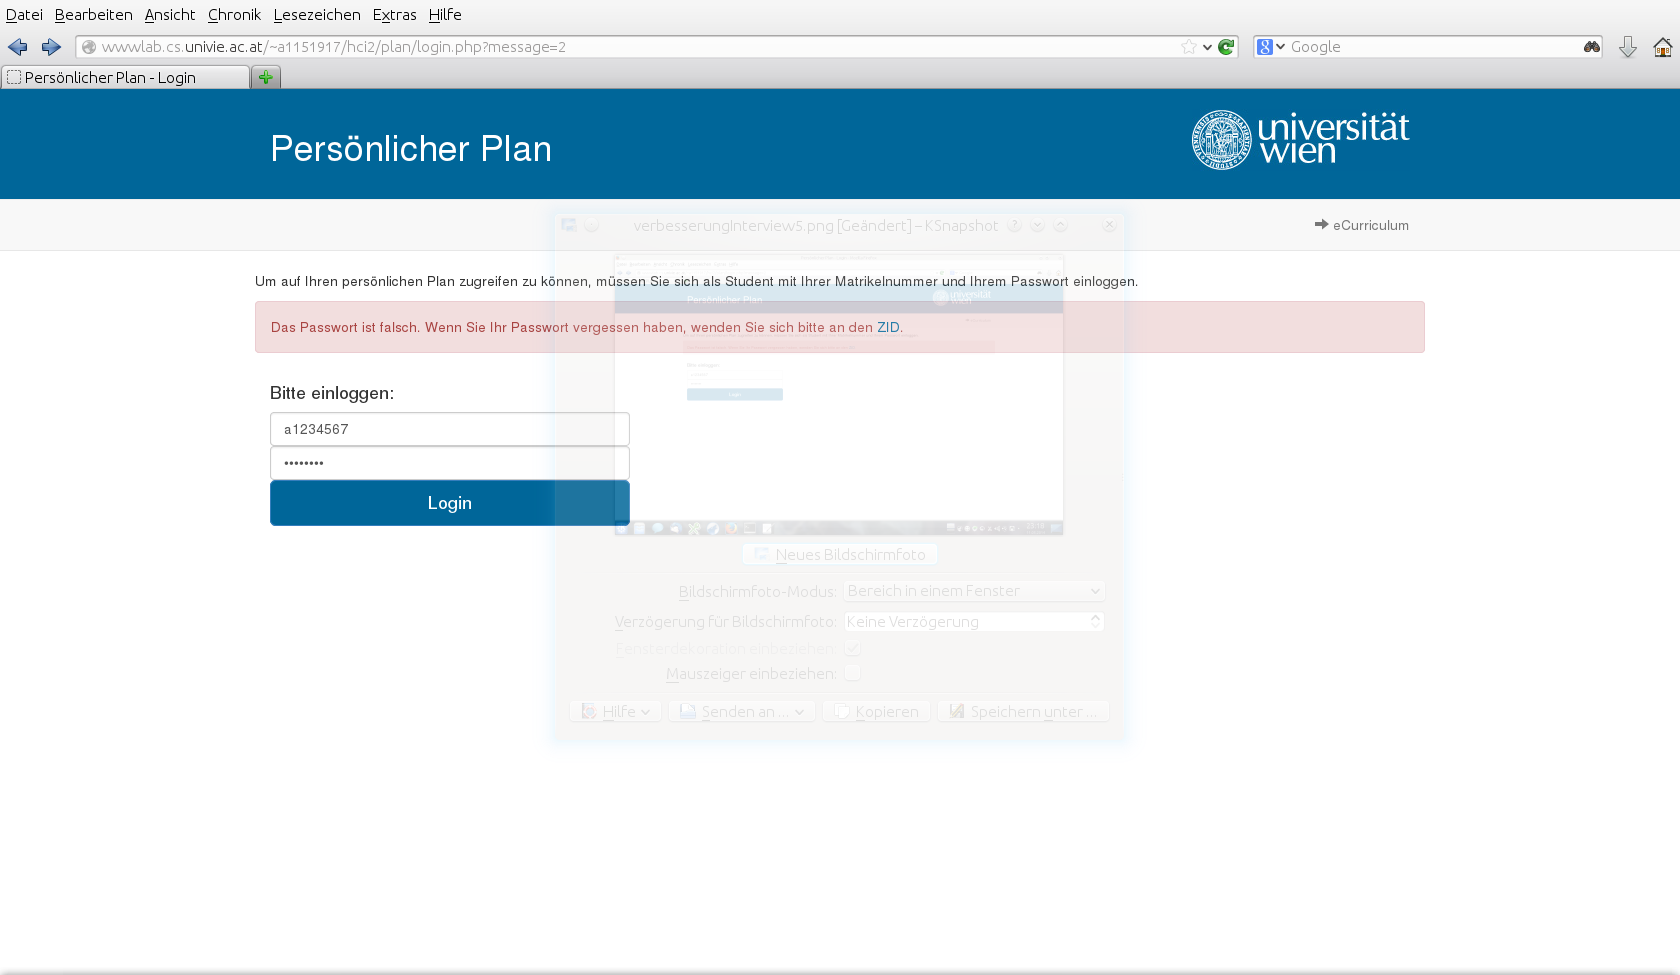
\includegraphics[width=\textwidth]{./verbesserungfehlermeldung1.png}}
\medskip


\noindent\makebox[\textwidth]{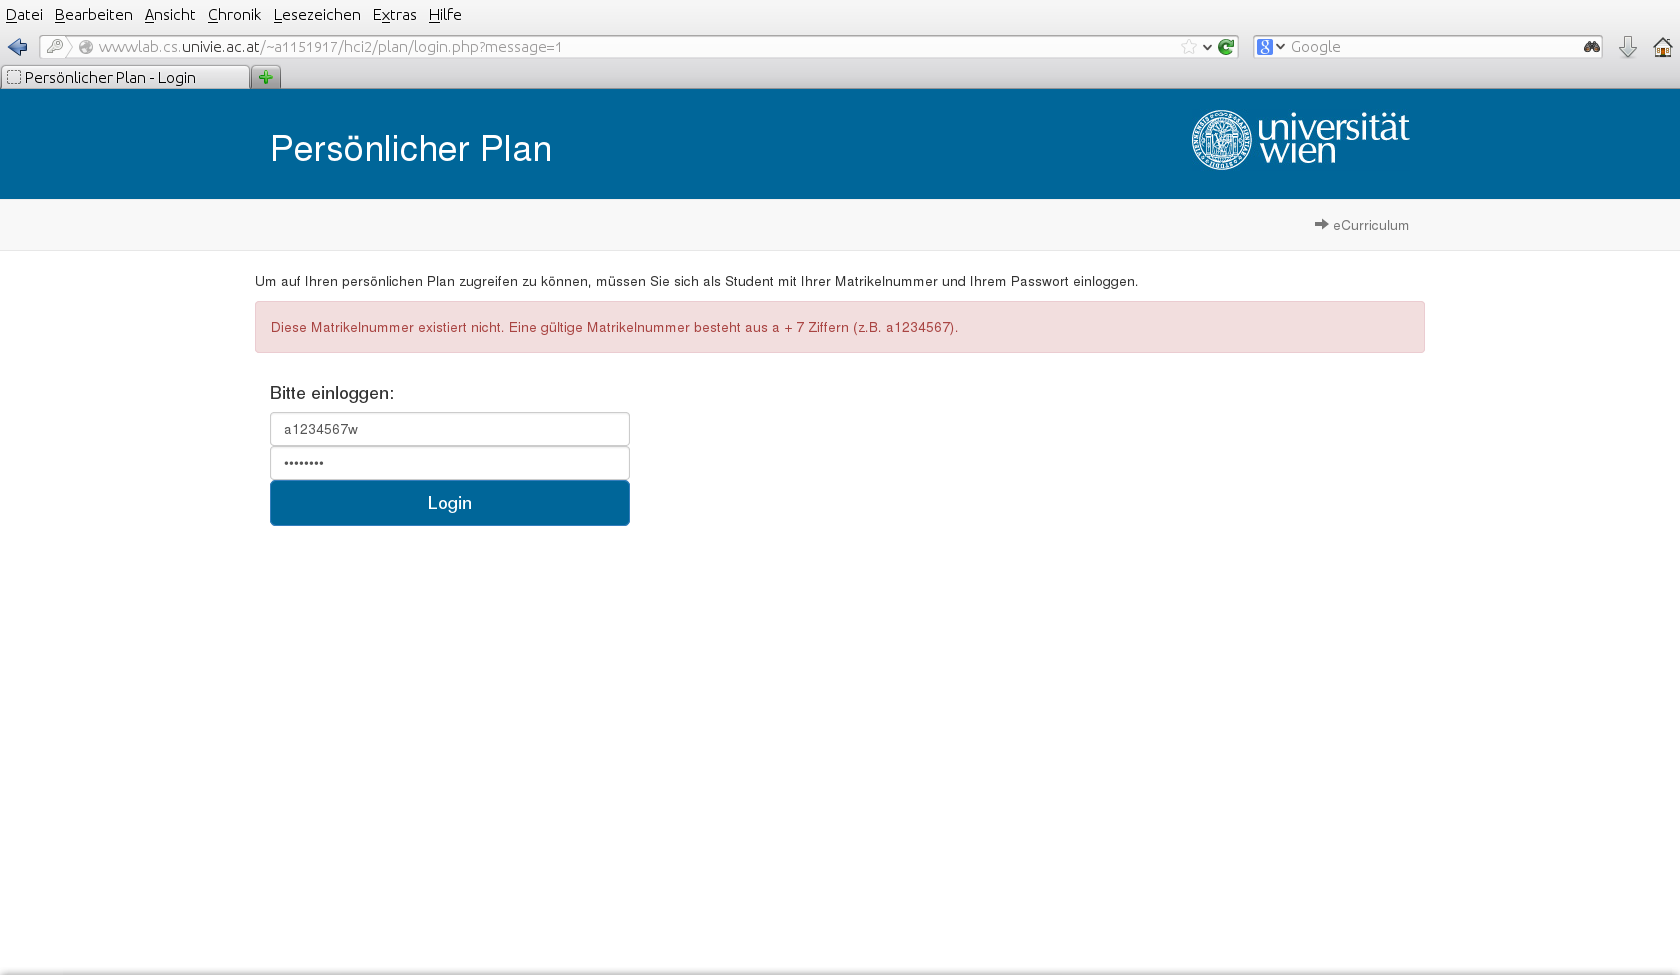
\includegraphics[width=\textwidth]{./verbesserungfehlermeldung2.png}}
\medskip


\noindent\makebox[\textwidth]{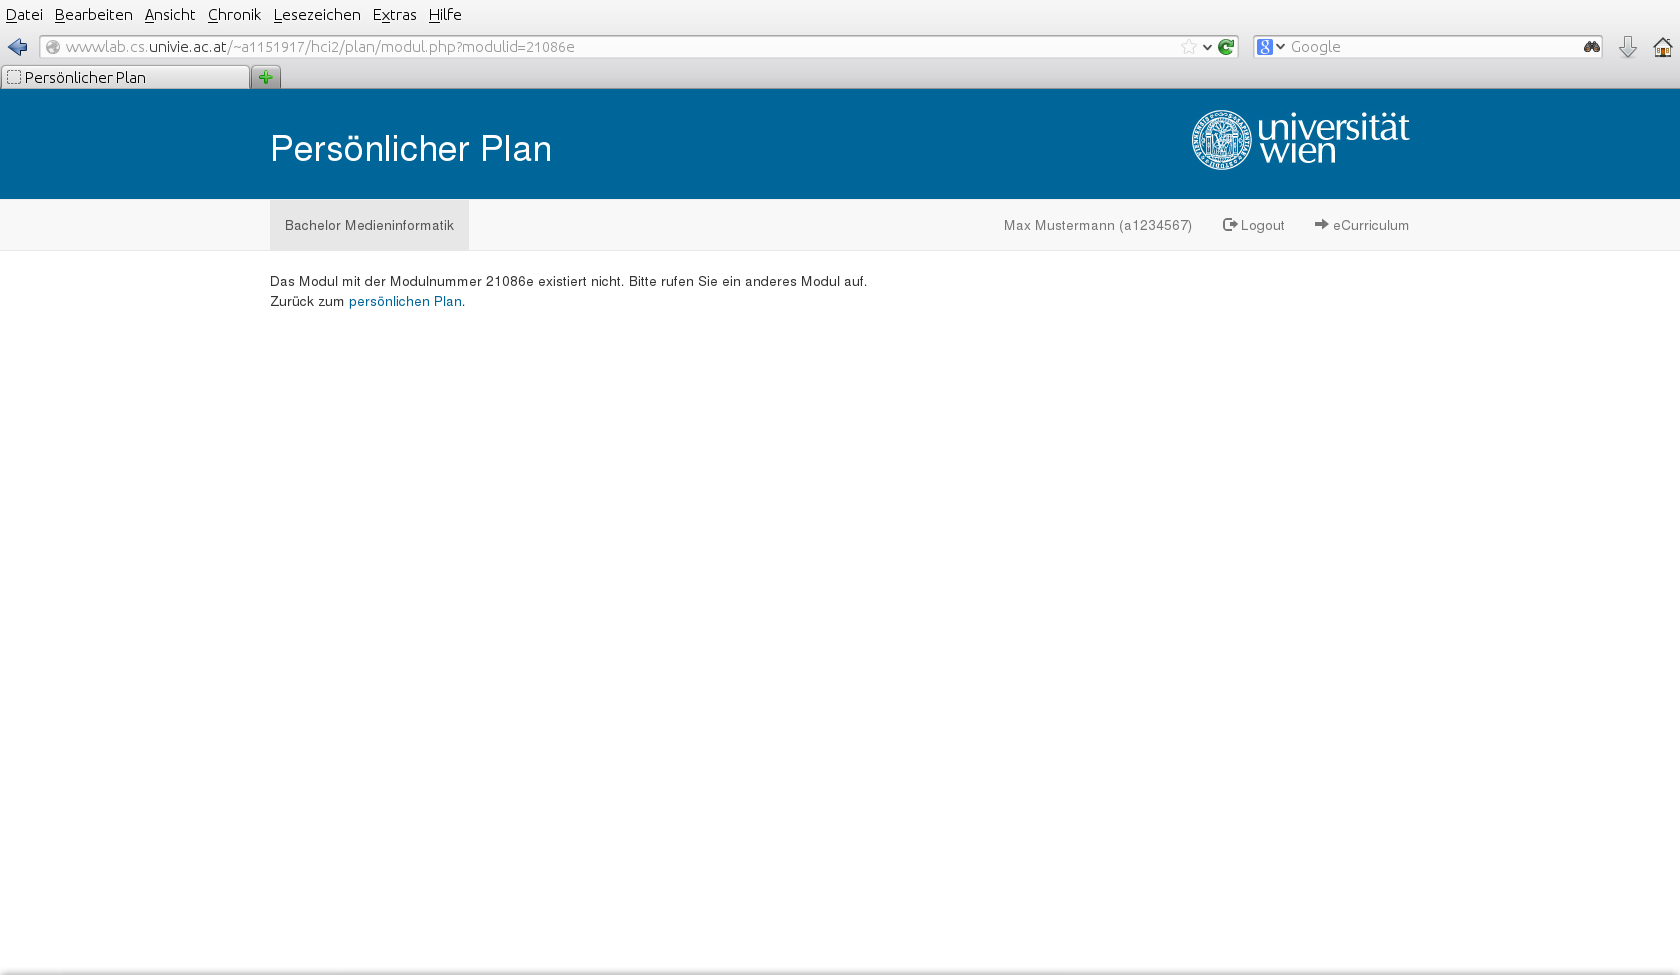
\includegraphics[width=\textwidth]{./verbesserungfehlermeldung3.png}}
\medskip

\subsection{Weiterentwicklung nach der Präsentation}

\subsubsection*{Statistik mit Anzahl der jeweiligen Noten}

Es gibt jetzt eine Statistik, in welcher zusätzlich die Anzahl der erbrachten Noten angezeigt wird.

\noindent\makebox[\textwidth]{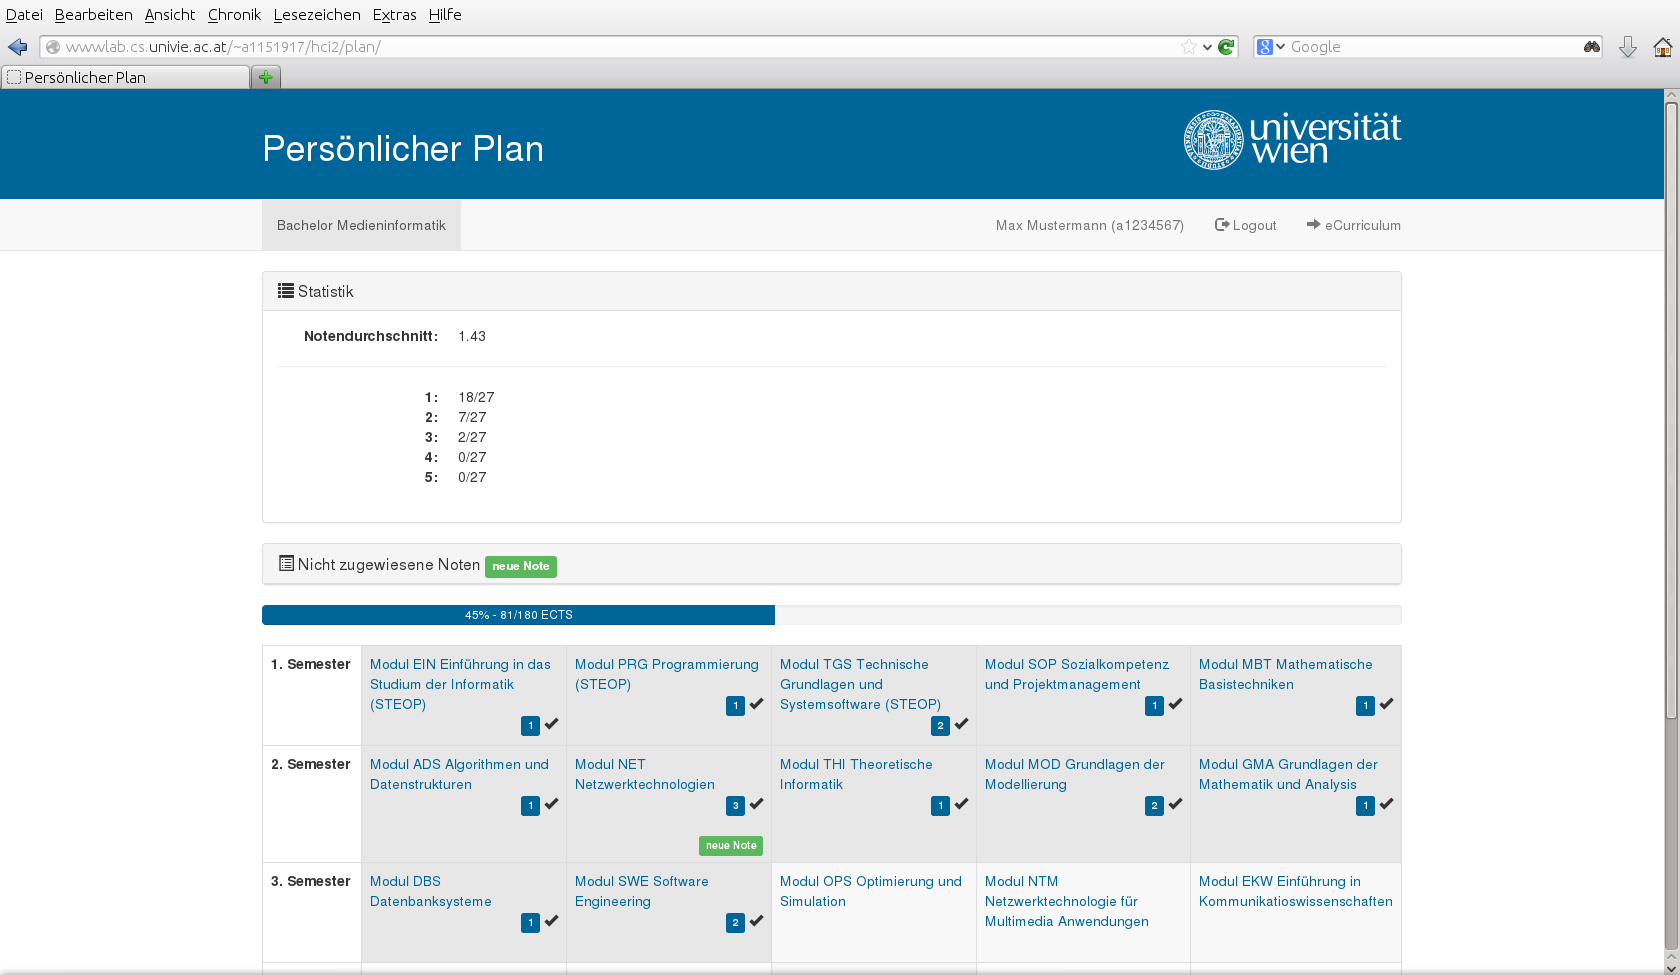
\includegraphics[width=\textwidth]{./verbesserung1.png}}
\medskip

\subsubsection*{Verlinkung zur Anmeldung zur Lehrveranstaltung}

Wenn eine Lehrveranstaltung noch nicht absolviert wurde, wird direkt ins Vorlesungsverzeichnis zum jeweiligen Modul verlinkt.

\noindent\makebox[\textwidth]{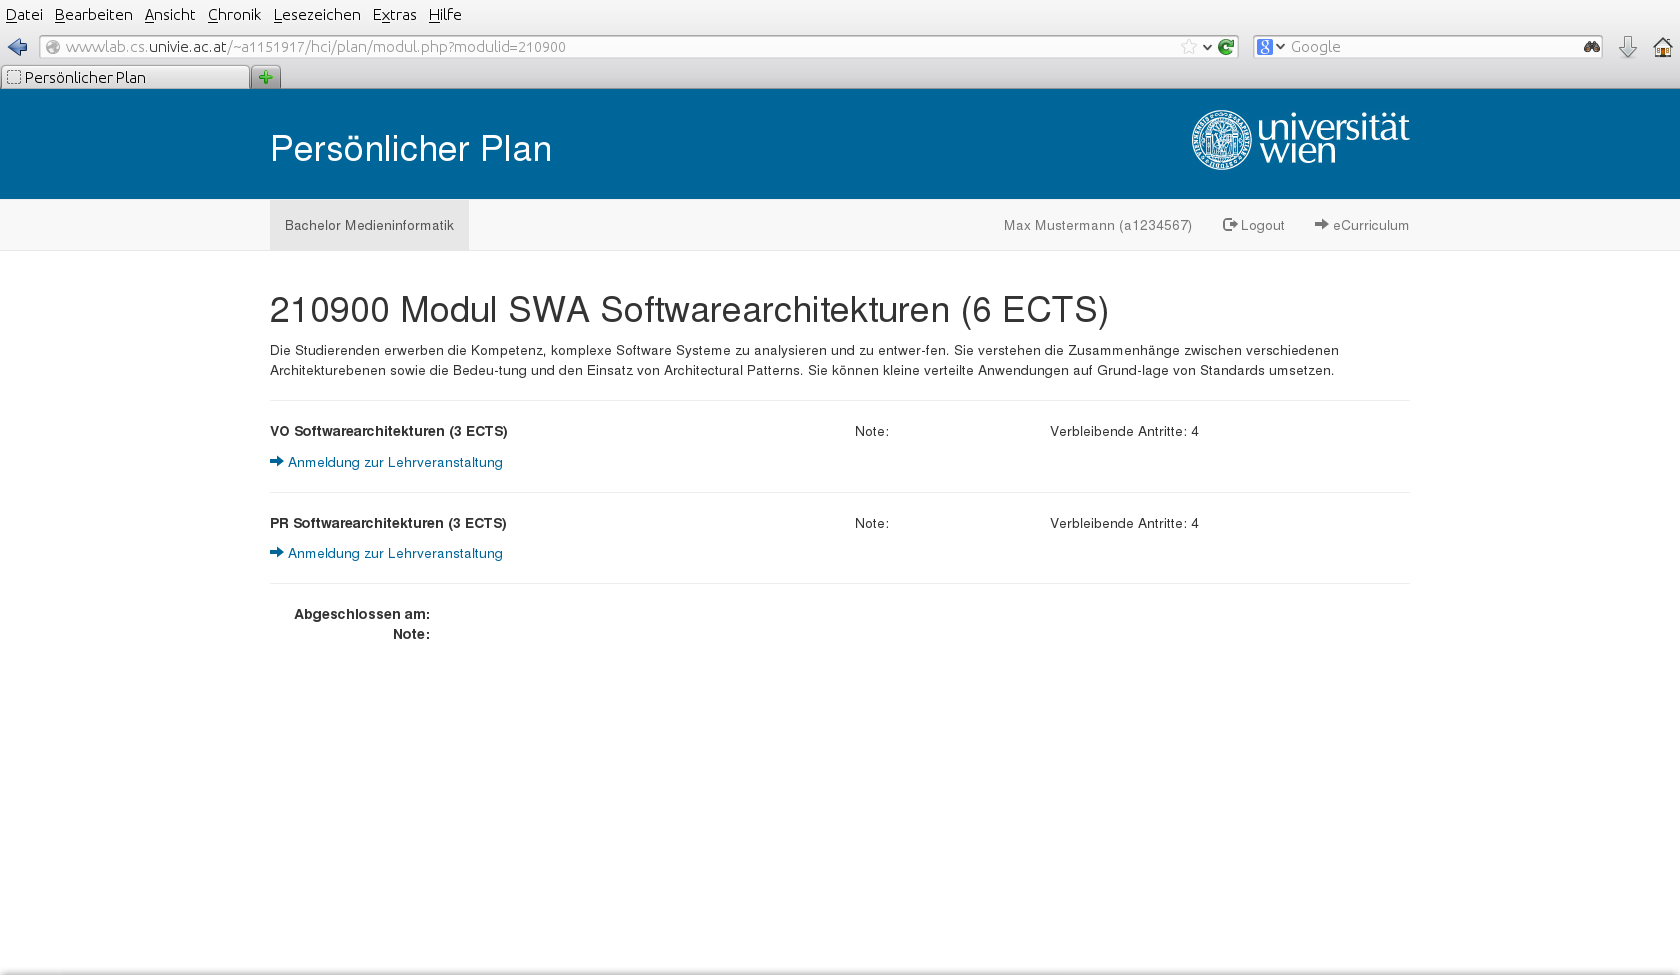
\includegraphics[width=\textwidth]{./verbesserung2.png}}
\medskip

\subsection{Weiterentwicklung nach dem Interview}

\subsubsection*{Kennzeichnung der STEOP im eCurriculum}

Da Probleme dabei auftraten, die für die STEOP relevanten Module zu erkennen, und dies auch als Verbesserung vorgeschlagen wurde, wird die STEOP jetzt auch in der
Semesteransicht hervorgehoben. Außerdem wurde eingebracht, dass die Information zur STEOP zu schlecht ersichtlich ist, weshalb die Information zur STEOP jetzt
schon beim Aufruf aufgeklappt ist.

\noindent\makebox[\textwidth]{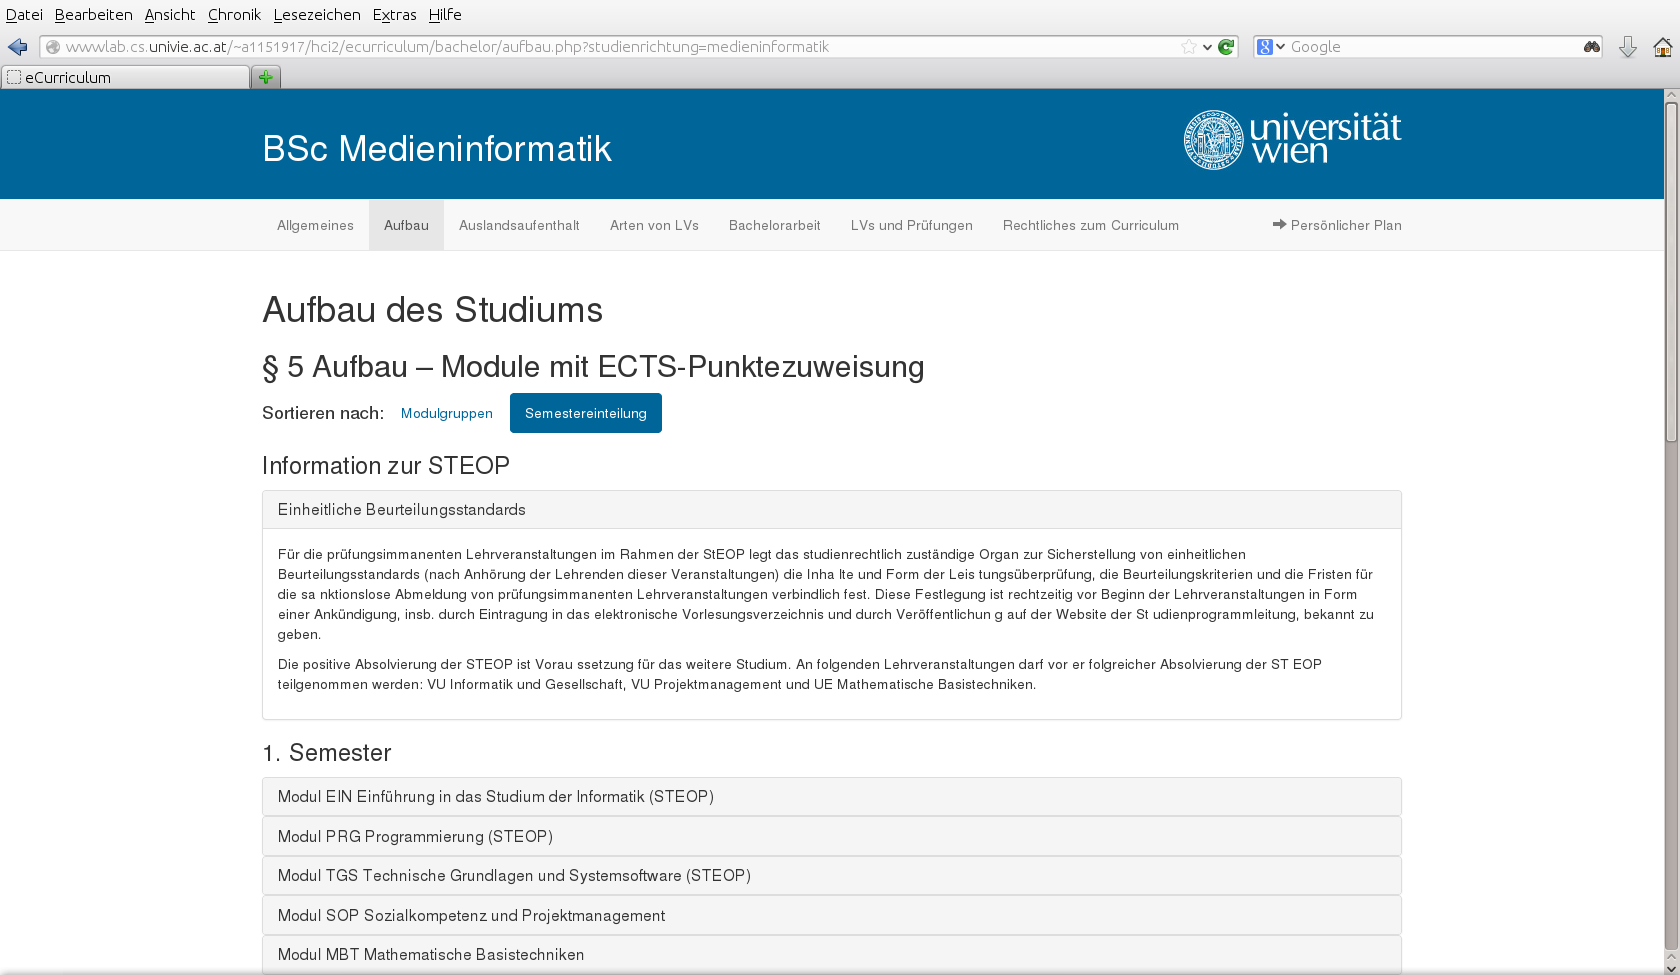
\includegraphics[width=\textwidth]{./verbesserungInterview1.png}}
\medskip

\subsubsection*{Linkbezeichnungen im eCurriculum}

Es wurden Linkbezeichnungen gewählt, die besser den Nutzen des jeweiligen Links ersichtlich machen (z.B. statt Ausland Auslandsaufenthalt).

\noindent\makebox[\textwidth]{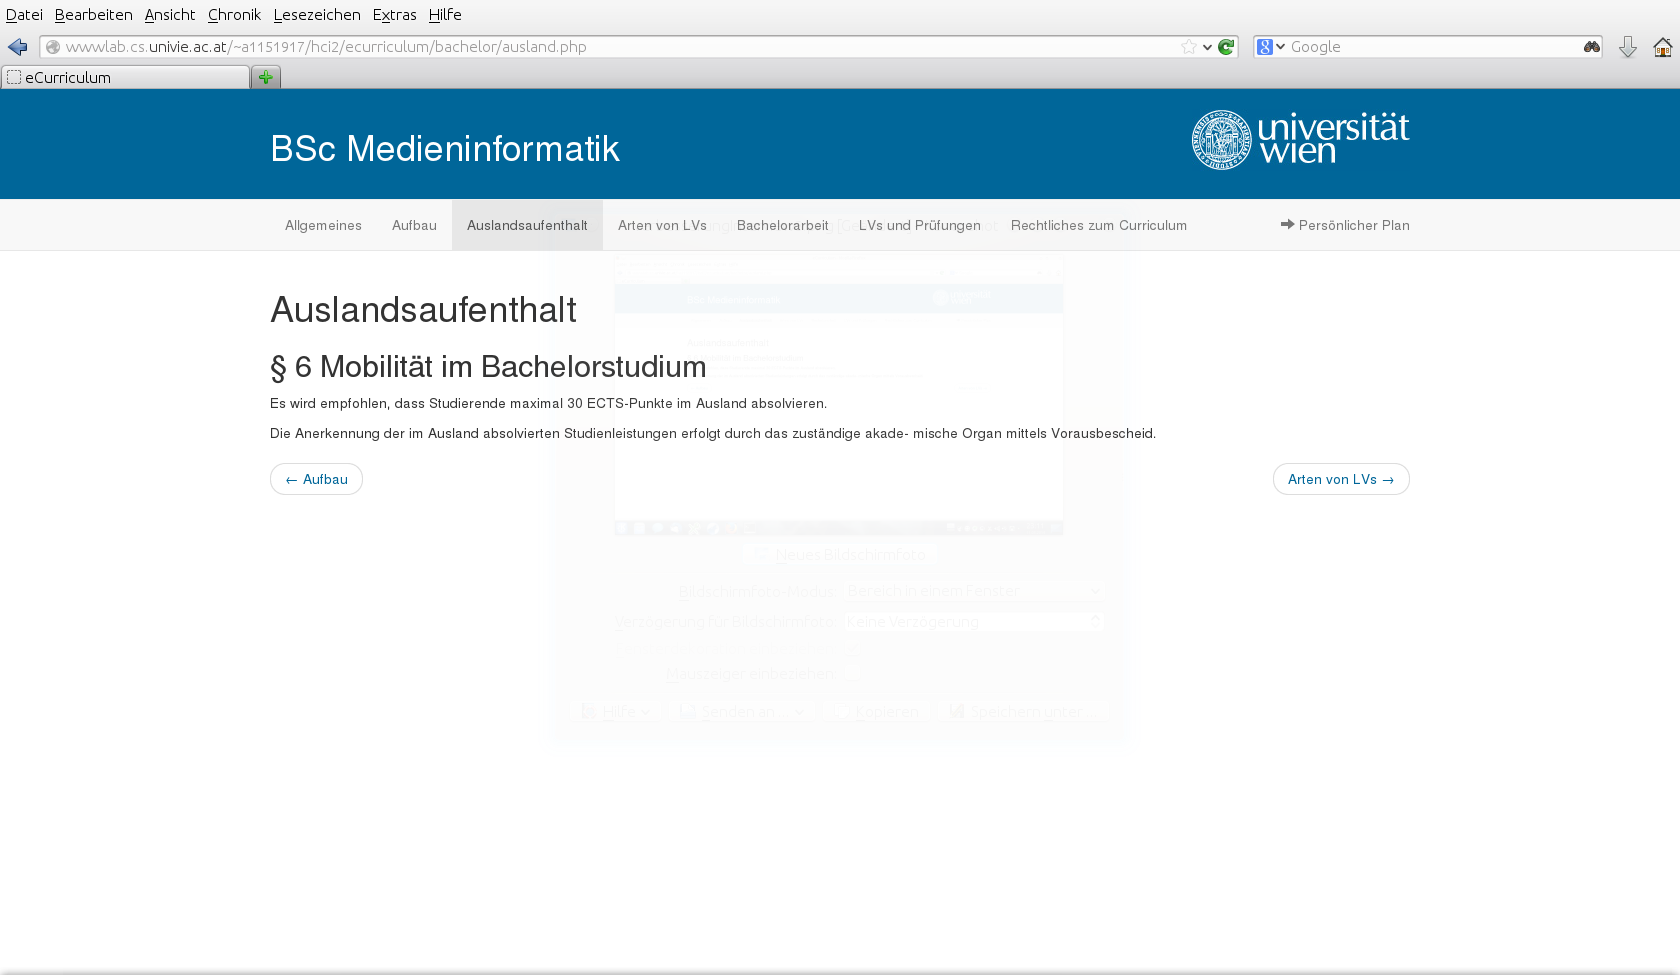
\includegraphics[width=\textwidth]{./verbesserungInterview2.png}}
\medskip

\subsubsection*{Nicht zugewiesene Noten im persönlichen Plan}

Nicht einem Modul zugewiesene Noten, die aber einem Studium (z.B. als Interessensmodul) zugewiesen sind, werden jetzt auch im persönlichen Plan in einem auklappbaren Fenster angezeigt.

\noindent\makebox[\textwidth]{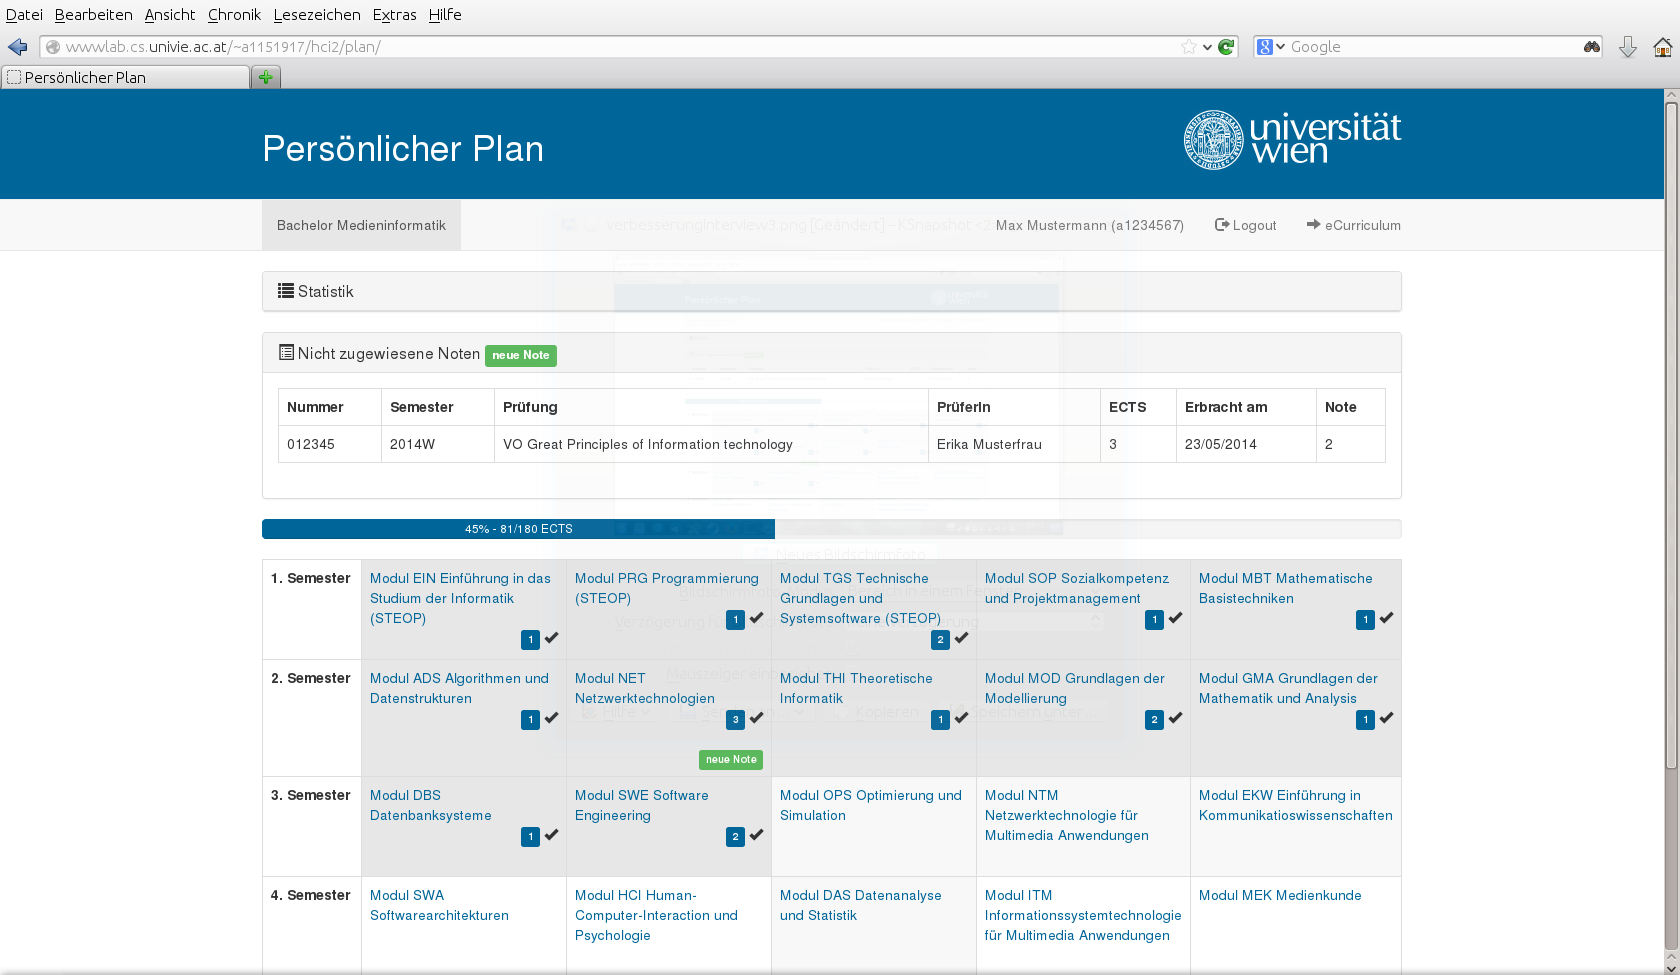
\includegraphics[width=\textwidth]{./verbesserungInterview3.png}}
\medskip

\subsubsection*{Kennzeichnung neuer Noten}

Die graue Kennzeichnung einer neuen Note war nicht immer ersichtlich, weshalb die neuen Noten jetzt in grün gekennzeichnet werden.

\noindent\makebox[\textwidth]{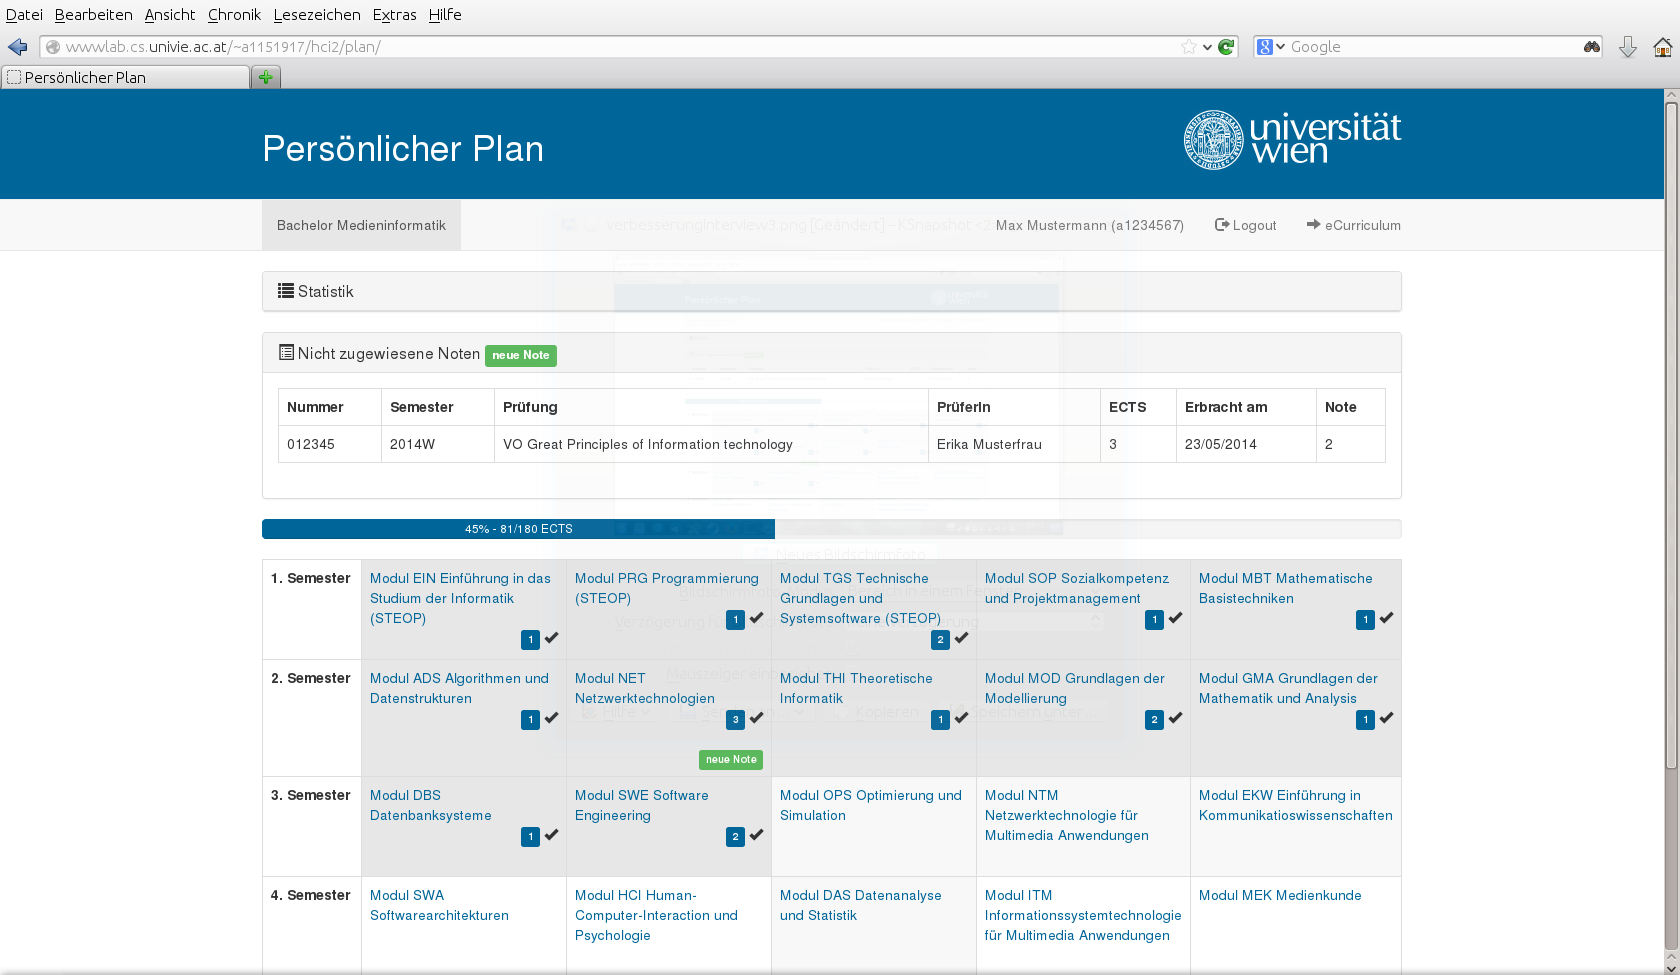
\includegraphics[width=\textwidth]{./verbesserungInterview3.png}}
\medskip

\subsubsection*{Notentabelle in der Modulansicht}

Die einzelnen Prüfungsantritte und die zugehörigen Noten werden in der Modulansicht jetzt in einer Tabelle dargestellt. Dadurch soll die Modulansicht übersichtlicher werden. Auch wird
die Modulnote als ``Modulnote'' gekennzeichnet.

\noindent\makebox[\textwidth]{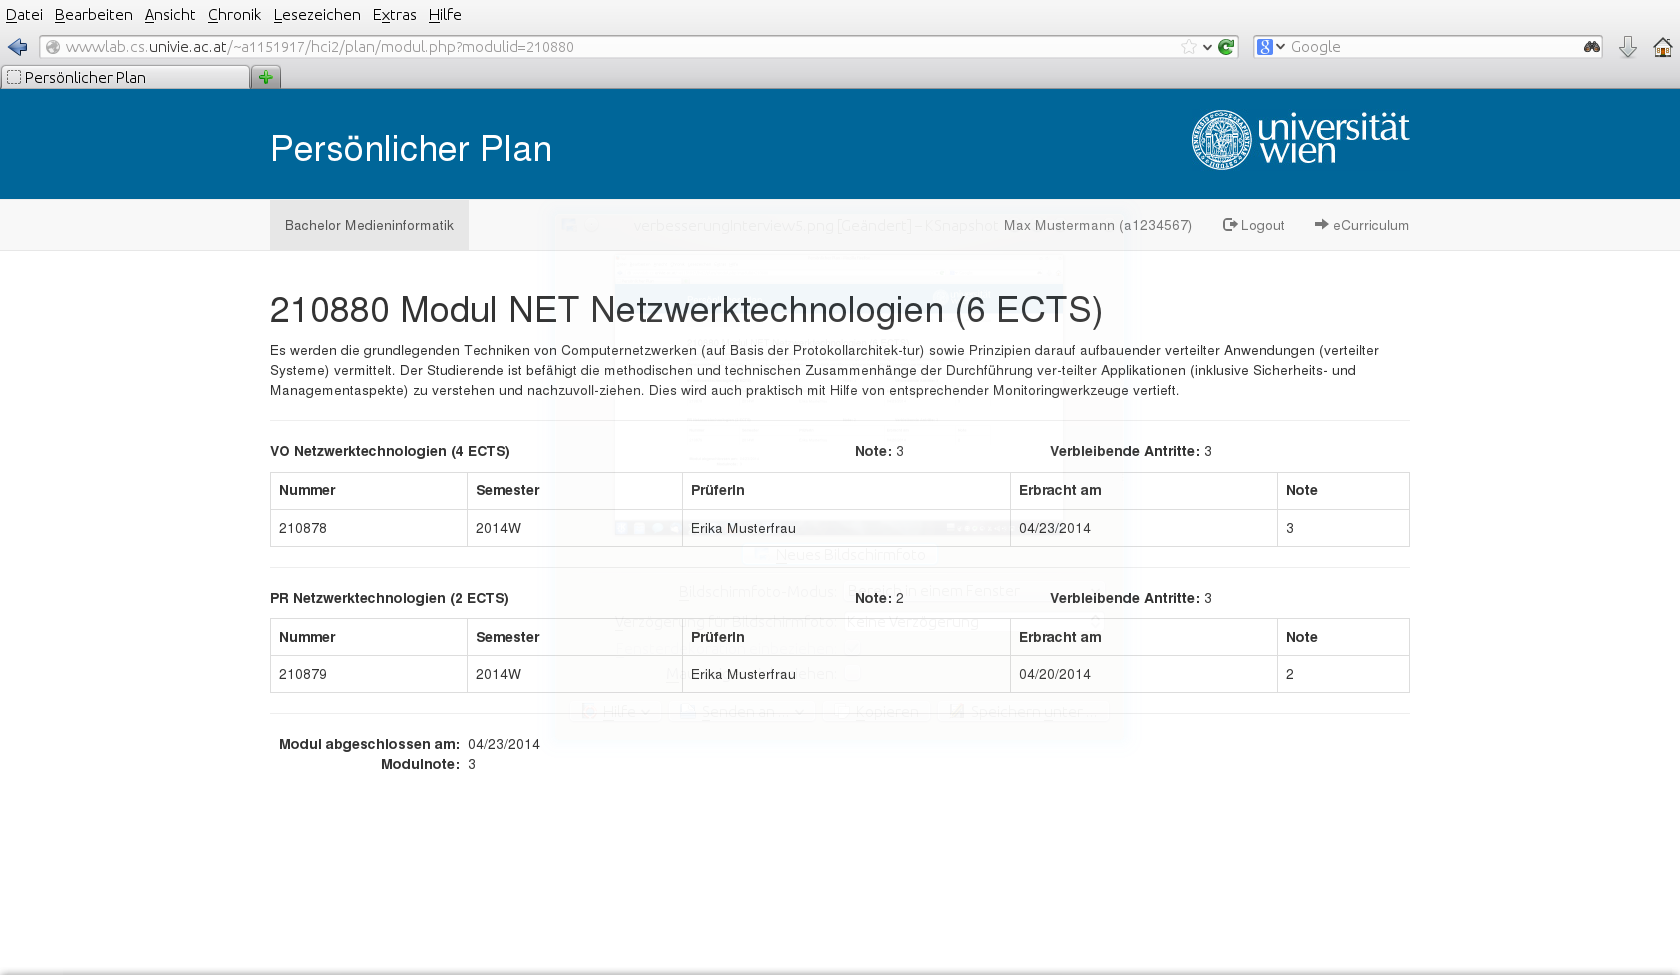
\includegraphics[width=\textwidth]{./verbesserungInterview4.png}}
\medskip



\section{Fragebögen}

\begin{description}
 \item[Datei auf cewebs:]Meilenstein 3 -- Team 1 -- Fragebögen
\end{description}

\end{document}
